\chapter{Technisch onderzoek}

Mijn technisch onderzoek startte bij het lezen van “The book” een boek over de taal Rust geschreven
door Steve Klabnik, Carol Nichols en met contributies van de Rust community. Tijdens het lezen
volgde ik de kleine code voorbeelden mee in een eigen Github repository. Dit maakte het makkelijker
om de geavanceerde hoofdstukken goed te begrijpen. 

Na een paar hoofdstukken diep in het boek was het tijd om de geleerde zaken tot de test te brengen.
De opdracht was om de miniversie van het gekende Linux commando grep te maken. Zo kon ik mijn kennis
over structs, ownership, enums en pattern matching, error handling, lifetimes en tests praktisch
toepassen.  

Op het einde van het boek was er een finaal project dat ook de laatste hoofdstukken bevatte. Het
project was het bouwen van een “simpele” multi-threaded server. Daar lag de focus op het werken met
meerdere threads, wat niet voor de hand ligt als je rekening moet houden met het geheugen. 

Na de taal onder de knie te hebben, begon ik met het leren van WebAssembly. Mits het nog een
piepjonge technologie is was er al heel wat documentatie/artikelen over te vinden op het web. Zo
begon ik bij de documentatie van Mozilla waar alles te vinden was om van start te gaan. Met
doorverwijzingen naar hun uitstekende geschreven blogposts die dieper gaan op hoe WebAssembly werkt. 

Vervolgens heb ik een keuze moeten maken welke frameworks ik zou gebruiken voor zowel front als
backend. Na wat onderzoek dat beschreven staat in “Welke front- end backend frameworks zijn er ter
beschikking?” heb ik gekozen voor Yew als frontend en Actix.web samen met diesel.rs als backend
framework.

\clearpage

\section{Omschrijving}

Om de huidige status van Full Stack web development in te onderzoeken heb ik gekozen voor een speed
typing test webapp te maken.

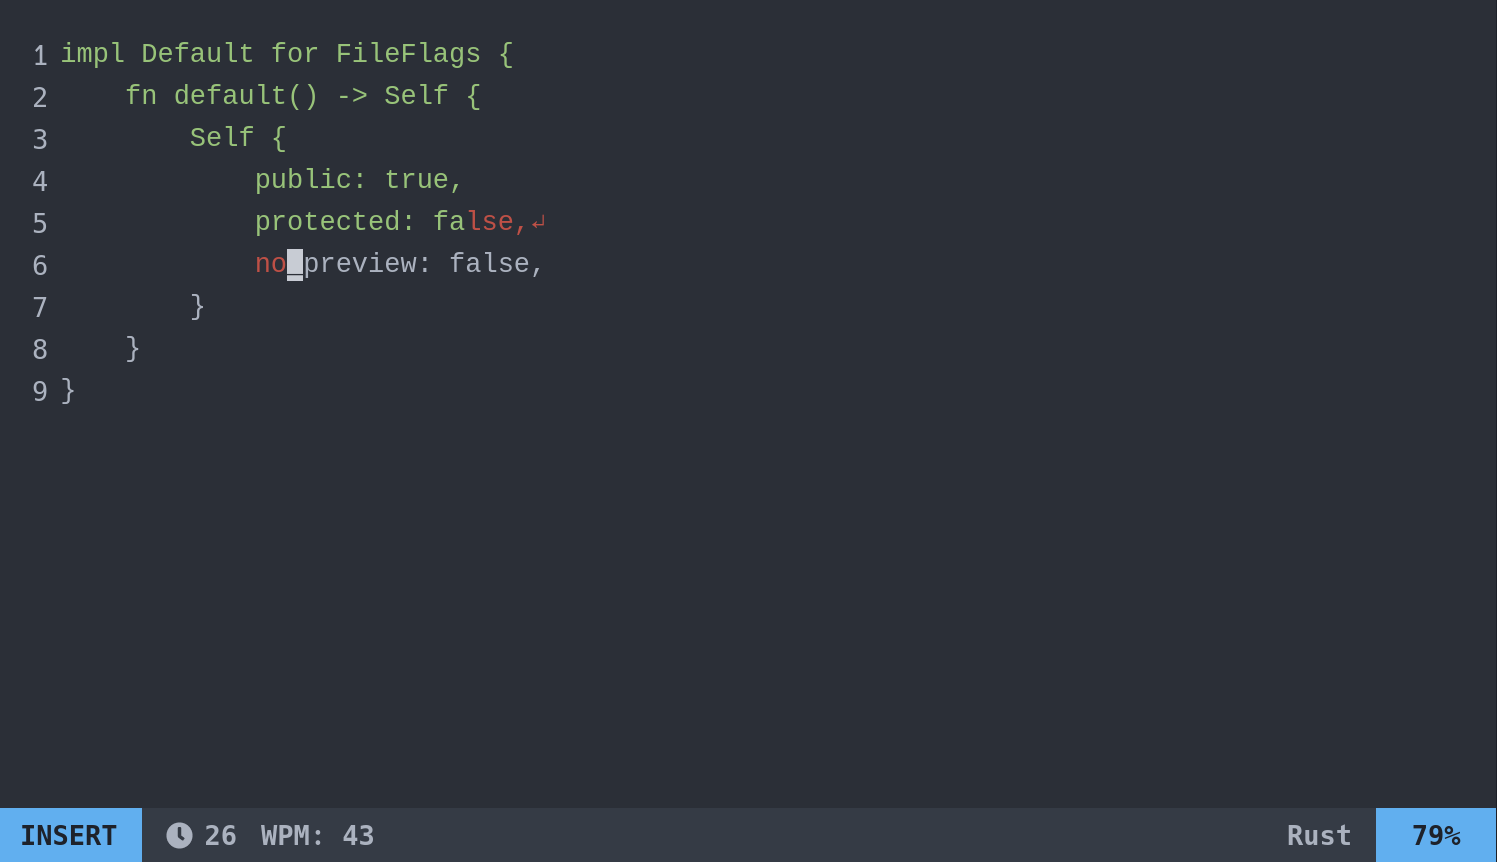
\includegraphics[width=\textwidth]{./figures/vim.png}

Het is een simpele applicatie waarbij de gebruiker een random code snippet krijgt die hij zo snel
mogelijk moet overtypen. Tijdens het typen wordt er live zijn tijd en words per minute (WPM)
bijgehouden. Als de gebruiker de volledige snippet heeft overgetypt krijgt hij een resultaten pagina
te zien. Daar kan hij zijn statistieken bekijken zoals: WPM, verlopen tijd, accuraatheid en het
aantal fouten. Daarna kan de gebruiker opnieuw spelen door op de letter ‘r’ in te drukken. 

\begin{wrapfigure}{l}{0.5\linewidth}
  \centering
  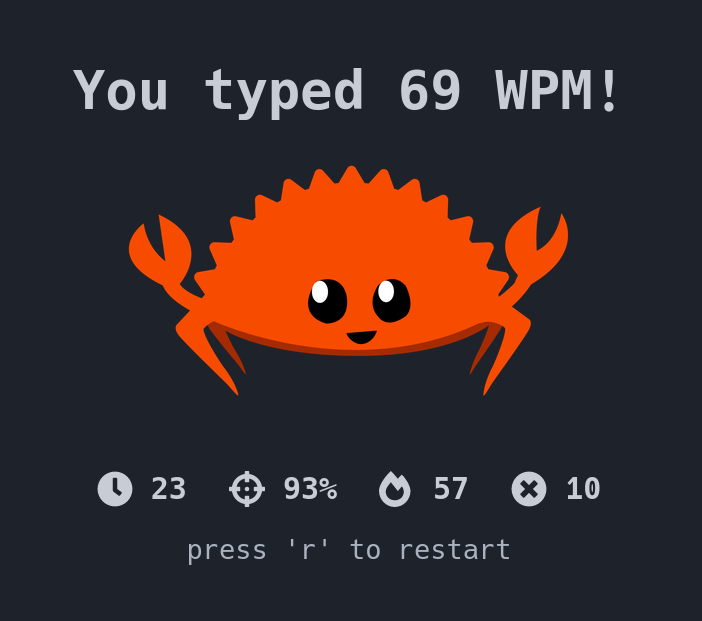
\includegraphics[width=0.78\linewidth]{./figures/result.png}
\end{wrapfigure}


Ik had voor ogen om bij dit project nog een aantal features eraan toe te voegen. Zoals authenticatie
met SSO, de statistieken opslaan in de database zodat er een lijn grafiek kon getoond op basis van
de historiek, andere database, profiel pagina, ci/cd enz. Helaas ben ik daar niet toe tot geraakt.
Het leren van Rust en WebAssembly nam meer tijd in beslag dan verwacht. Sinds ik geen voorkennis had
van Rust of een gelijkaardige systeem level programmeertaal was dit project al een hele uitdaging op
zich.

\clearpage

\section{Opbouw/structuur}

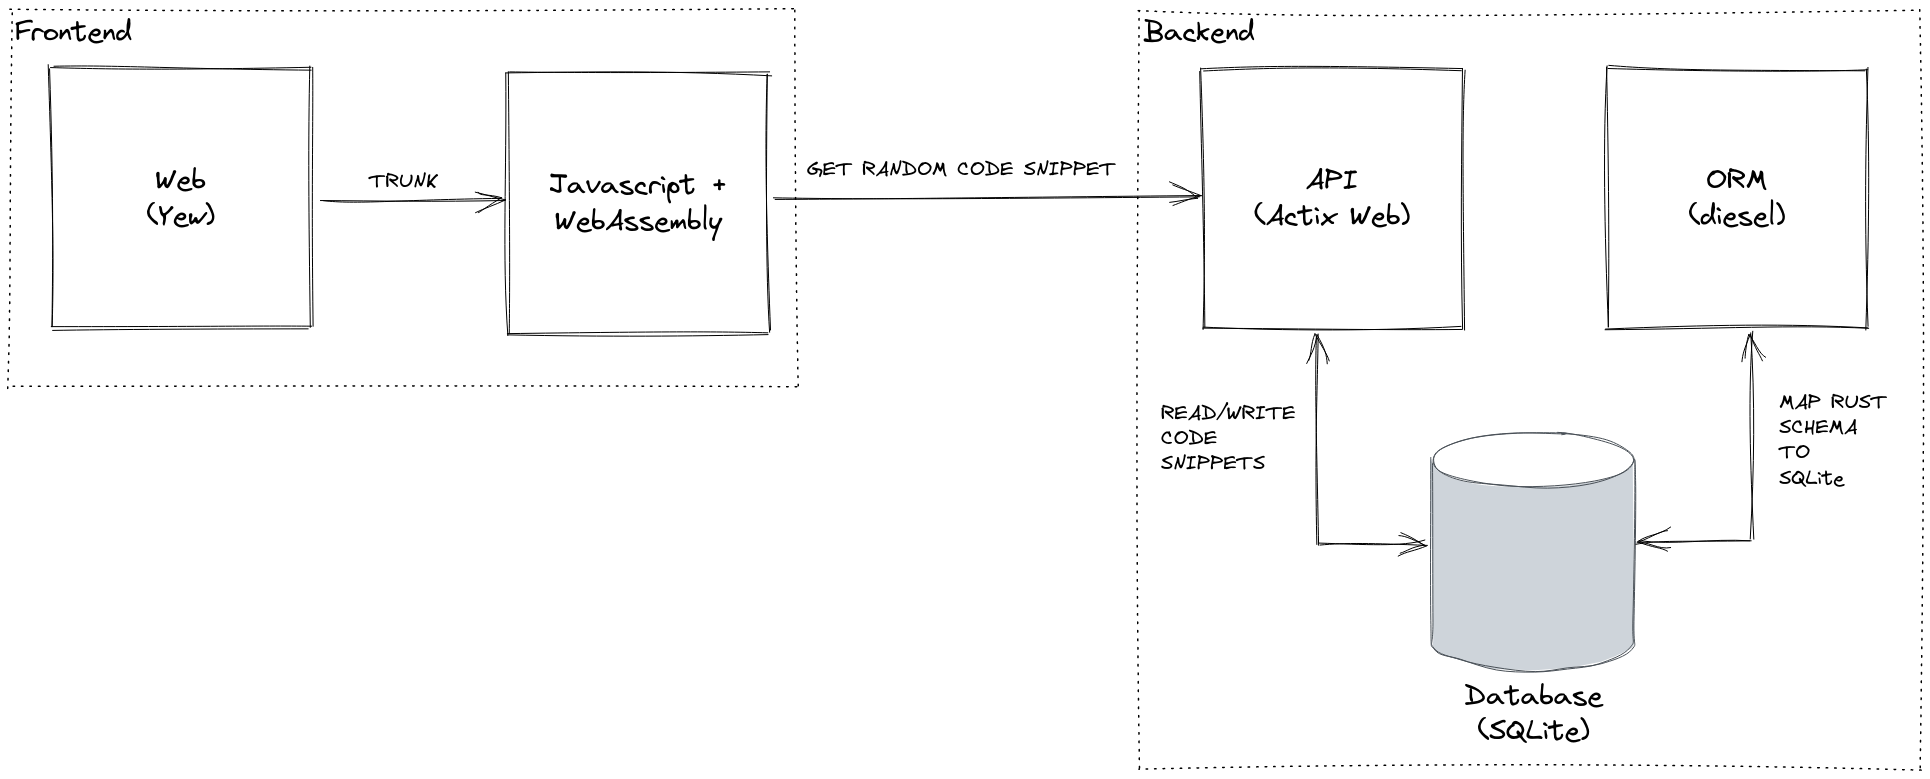
\includegraphics[width=\textwidth]{./figures/structuur.png}

De frontend van de applicatie is volledig geschreven in Rust. Dit is mogelijk gemaakt door het
gebruik van Yew als framework. Daarbij heb ik Tailwindcss gebruikt als CSS framework. Tailwindcss is
een utility-first CSS framework om snel custom user interfaces te bouwen. Samen met een component
based framework als Yew hoeft ik zelf geen CSS meer schrijven maar kan ik direct tailwindcss zijn
utility classes toepassen op mijn components. Wat maakt voor een geweldige developer experience. 

Om alles van frontend te kunnen compileren en uitvoeren heb ik trunk gebruikt. Trunk is een WASM web
applicatie bundelaar. Het gebruikt een eenvoudige config voor het bouwen en bundelen van WASM, JS
snippets en andere assets (images, css, scss) via een source HTML bestand. Met een simpel commando
als \mintinline{bash}{trunk build} bouwt hij de hele frontend en met \mintinline{bash}{trunk serve
--serve} draait hij de lokale dev server.  

Bij het laden van de startpagina haalt de frontend een random code snippet op via de API. De API
haalt de snippets op uit een SQLite database. Om de database in sync te houden met de Rust code werd
er diesel gebruikt als ORM framework.


\section{Werking frontend}


\includegraphics[width=\textwidth]{./figures/components.png}

De startpagina is geïnspireerd door mijn favoriete editor vim. Zo krijg je een simpele versie van
vim te zien als editor voor het typen. Hieronder zie je een schema van de compositie van de
belangrijkste componenten.

Game: rendert op basis van de game status Vim of Result 
Vim: de tekst editor voor de code en bevat Window \& StatusLine als children 
Window: rendert de tekst samen met LineNumber 
StatusLine: toont live statistieken zoals de huidige taal, tijd, WPM, progress 
Result: toont alle statistieken op het einde van de game

Het bouwen van de interface was redelijk eenvoudig, maar om de speed typing test te doen werken was
het verassend moeilijk. Om de gebruiker het idee te geven dat hij tekst over typt heb ik vier html
elementen gebruikt: een cursor met het huidige karkater, de correct getypte tekst, de foute getypte
tekst en de resterende tekst.

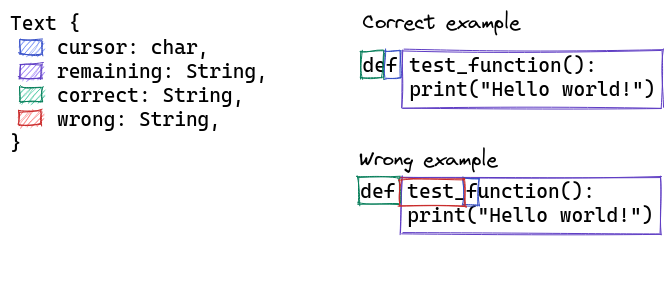
\includegraphics[width=\textwidth]{./figures/text.png}

Bij elk keypress event wordt er gecontroleerd of de key gelijk is aan het volgende karakter. Indien
het gelijk is wordt het huidige karakter van de cursor toegevoegd aan de string met de correcte
karakters en de cursor schuift een karakter op. Hetzelfde geldt als men een verkeerde key indrukt
maar de cursor wordt dan toegevoegd aan de string met de foutieve karakters. Als de gebruiker de
“Backspace” toets indrukt kan hij zijn foute karakters verwijderen tot de string leeg is. 

Dit was het basisidee waarmee ik aan de slag ging. De moeilijkheid van het bouwen lag vooral aan hoe
ik efficiënt de variabelen van de tekst en de bijhorende statistieken in een state kan opslaan zodat
elk component slechts rendert als het nodig is.  

Mijn eerste oplossing was het gebruik van globale state met de \mintinline{rust}{use_reducer}
hook. Als je vertrouwd bent met React zijn de meeste hooks zoals \mintinline{rust}{use_reducer},
\mintinline{rust}{use_state}, \mintinline{rust}{use_effect} overgenomen in Yew. Indien niet leg
ik het kort even uit. Voor simpele variabelen op te slaan in een state zoals bijvoorbeeld een
boolean gebruik je de \mintinline{rust}{use_state} hook. Die zorgt ervoor dat de boolean doorheen
het component lifecycle hetzelfde blijft tenzij je hem aanpast. Als je hem aanpast dan zal het
component opnieuw renderen.  

De \mintinline{rust}{use_reducer} hook werkt gelijkaardig maar wordt gebruikt voor complexere
states. Zo komt het met een dispatch functie die een argument neemt van het type Action. Wanneer
deze wordt aangeroepen, worden de actie en de huidige waarde doorgegeven aan de reducer functie die
een nieuwe state berekent en retourneert.

Zo heb ik 5 acties gedefinieert: \mintinline{rust}{NewSnippet}, \mintinline{rust}{Keypress},
\mintinline{rust}{Backspace}, \mintinline{rust}{Tick} en \mintinline{rust}{Reset}. In die acties zit
de meeste logica van het spel en kan gebruikt worden in components om de state van het spel aan te
passen. 

Het probleem met de \mintinline{rust}{use_reducer} hook is dat een component de hele state opneemt.
Als de child components een variabel nodig hebben van de state, moeten die als properties worden
doorgeven. Hier is niks mis mee tenzij je een diep genest child component hebt die afhankelijk is
van de state. Dan heb je “prop drilling” waarbij je vanuit de parent component de props moet
doorgeven aan zijn children die dezelfde props dan doorgeven aan hun children, en zo verder tot dat
je bij de gewenste component bent.


\centering

\includegraphics[width=0.6\textwidth]{./figures/use_reducer.png}



Dit heb ik opgelost door de \mintinline{rust}{use_context} hook te gebruiken samen met de
\mintinline{rust}{use_reducer}. Zo kon ik een \mintinline{rust}{GameStateProvider} component
definiëren die de context (state) consumeert en gebruikt kan worden door alle child components. Dit
betekent dat ik de props niet meer hoefde te “prop drillen” maar direct kon aanspreken vanuit alle
child components onder de GameStateProvider. Helaas heeft deze methode ook zijn nadelen: 
\begin{itemize}
    \item als de state gebruikt wordt in een child component moet de hele state gekloond worden 

    \item stel een child component gebruikt een variabele A van de globale state, als de hele state
    wordt aangepast behalve de variabele A zal het child component toch onnodig re-renderen. 
\end{itemize}

Zo ben ik uiteindelijk geland op yewdux een state management library voor Yew die werkt met een
globale store/state. Het is verglijkbaar met de populaire React library Redux. Yewdux gebruikt een
CoW (clone on write) managementstrategie. Dit betekent dat de state bij elke mutatie een keer wordt
gekloond. Door het op deze manier te doen kunnen we beknopt een precieze mutatie uitdrukken zonder
extra boilerplate, en gebruik maken van change detection om onnodige re-renders te voorkomen. 

Een voorbeeld hiervan is de \mintinline{rust}{use_selector} hook van yewdux, waarmee we een
variabele van de state kunnen selecteren en slechts re-renderen als de variabel verandert i.p.v. de
hele state.

De werking van de backend verschilt niet veel met het voorbeeld “Todo” applicatie die we gemaakt
hebben in “Hoe bouw je een API in Rust?”. Opnieuw werd er gekozen voor een simpele SQLite database
om de code snippets in op te slaan. Zoals eerder gezien wordt het database schema aangemaakt door
migrations uit te voeren met diesel CLI.  Dit is een database first aanpak, na wat onderzoek lijkt
het me dat diesel.rs jammer genoeg geen andere aanpakken ondersteund zoals code first. Met code
first kan je vanuit models die gedefinieerd staan in code automatisch migrations aanmaken die het
database schema aanpassen/aanmaken. 

In de speed typing database gebruiken we twee tabellen “languages” en “snippets”. Die een een op
veel relatie met elkaar hebben. De tabel languages bevat de soorten programmeertalen en de tabel
snippets de code. De code is hier gewoon opgeslagen als tekst in de tabel snippets. Het is wel
belangrijk dat de code geen spaties bevat maar tabs. Daarvoor heb ik kleine parser tool geschreven
om makkelijk code snippets te maken. Het neemt een tekstbestand als input en zet alle spaties en
enters om naar de respectievelijke karakters “\textbackslash t” en “\textbackslash n”. Zo kan de
frontend makkelijk de juiste enters en tabs weergeven. 

De API kent een aantal routes, ik lijst ze hier even op: 
\begin{itemize}
    \item GET, POST, DELETE  /languages
    \item GET, POST, DELETE /snippets 
    \item GET /snippets/random 
    \item GET /snippets/\{language\_id\}"
\end{itemize}

Uiteindelijk gebruikt de frontend maar een route “/snippets/random” om een random code snippet op te
halen uit de database. Om ervoor te zorgen dat we niet eerst alle snippets op halen uit de database
om dan een random snippet eruit te selecteren. Heb ik eerst via een SQL-query de snippets tabel
random gesorteerd en het eerste resultaat eruit gepakt.  

Standaard zal Rust of diesel het random type niet kennen. Gelukkig voorziet diesel de
\mintinline{rust}{no_arg_sql_function} macro waarmee je SQL functies kunt mappen naar Rust types.

Zo kan ik het random type importeren vanuit het schema en gebruiken in mijn SQL-query opgesteld door diesel.

\section{Werking backend}
